\chapter{Projeto de Software}
\label{cap:06}

Este capítulo apresenta a arquitetura técnica e as especificações de projeto que fundamentam o sistema de gerenciamento de coleções. Nele, detalham-se as interfaces, a modelagem de dados e as regras de persistência utilizadas no desenvolvimento da aplicação.

\section{Projeto de Interface}
As interfaces do sistema foram projetadas na ferramenta \textbf{Figma} e adotam um partido visual deliberadamente simples, construído sobre poucos componentes reutilizáveis, uma tipografia única e uma paleta reduzida, ancorada em um tom de roxo. A escolha é coerente com a proposta do produto: como o conteúdo das fichas é inteiramente definido pelo usuário no editor de \textit{layouts}, a interface que o cerca deve permanecer discreta, para não competir visualmente com aquilo que o próprio usuário compôs. Convém registrar que os protótipos aqui descritos foram elaborados na fase de concepção, antes da implementação, e representam a intenção de projeto: definem a organização e o comportamento pretendidos para as telas, e não seu resultado final, que pode incorporar ajustes decorrentes do desenvolvimento.

O sistema divide-se em duas regiões visualmente distintas. Antes da autenticação --- na página inicial, no cadastro e nas telas de \textit{login} e de recuperação de senha ---, o conteúdo aparece centralizado e isolado, sem elementos de navegação, já que ainda não há acervo a percorrer. Após a autenticação, as telas passam a compartilhar uma mesma moldura: uma barra lateral fixa, que dá acesso às categorias do usuário e à área social; uma barra superior, que reúne a identificação da tela atual, o acesso às notificações e o menu do usuário; e a área central, onde o conteúdo é efetivamente apresentado.

A navegação pela hierarquia de três níveis é o eixo da área central. Categorias, coleções e itens são exibidos em uma grade de \textit{cards}, e uma trilha de navegação no topo indica a posição do usuário --- por exemplo, ``Categorias > Livros > Lidos'' ---, permitindo retornar a qualquer nível anterior com um clique. Os \textit{cards} adaptam-se ao que representam: os de coleção exibem o indicador de privacidade e a contagem de itens, enquanto os de item privilegiam a imagem de capa. Acima da grade situam-se os controles de modo de exibição, ordenação e filtro previstos nos requisitos, e um botão flutuante, no canto inferior, cria um novo registro no contexto em que o usuário se encontra.

O editor de \textit{layouts} recebeu tratamento próprio, por ser a tela em que a proposta da plataforma se materializa. Sua composição divide-se entre uma área de edição, que representa a ficha em construção, e um painel lateral com os tipos de Elemento disponíveis --- imagens, textos, classificações, datas, listas e formas ---, que o usuário arrasta para a área de edição e ali posiciona e redimensiona livremente. Uma alternância entre os modos de edição e de prévia permite verificar, sem sair da tela, como a ficha será exibida em modo leitura.

As telas de interação social seguem a mesma moldura. A área de amigos separa, em abas, os vínculos já estabelecidos e as solicitações pendentes, e oferece a busca por código de usuário ou por nome prevista no RF-20. No perfil de outro usuário, exibem-se os dados públicos e as coleções visíveis conforme o vínculo existente, cada uma acompanhada da ação de seguir ou deixar de seguir.

\section{Projeto de Dados}
A persistência de informações utiliza o Sistema Gerenciador de Banco de Dados (SGBD) \textbf{PostgreSQL 16}, executado em ambiente isolado através de \textbf{Docker}. A manipulação e a administração dos dados são realizadas por meio do \textbf{DBeaver}, cliente gráfico de administração de bancos de dados relacionais.

O banco de dados foi estruturado para suportar tipos de dados modernos e performáticos, incluindo:
\begin{itemize}
    \item \textbf{UUID (Universally Unique Identifier):} Utilizado para todas as chaves primárias e estrangeiras;
    \item \textbf{JSONB:} Para o armazenamento eficiente de configurações dinâmicas de interface;
    \item \textbf{Varchar(n):} Para cadeias de caracteres de tamanho limitado, com restrição imposta no nível do banco;
    \item \textbf{Text:} Para cadeias de caracteres extensas, sem limite explícito de tamanho;
    \item \textbf{Timestamp:} Para o registro cronológico de eventos e criações;
    \item \textbf{Float:} Para valores numéricos fracionários, utilizados em ajustes tipográficos;
    \item \textbf{Boolean:} Para o registro de estados binários (verdadeiro/falso);
    \item \textbf{Enum:} Para campos com domínio restrito a um conjunto pré-definido de valores.
\end{itemize}

\subsection{Mapeamento Objeto-Relacional}
O mapeamento entre o modelo de domínio (TypeScript) e o modelo relacional (PostgreSQL) é gerenciado pelo \textbf{Prisma ORM}. Para garantir a integridade dos dados e a fidelidade aos requisitos, adotaram-se as seguintes regras de mapeamento:

\begin{itemize}
    \item \textbf{Idioma dos identificadores:} Os nomes conceituais empregados no texto desta monografia estão em português (Elemento, TipoElemento, Categoria, Coleção), ao passo que os identificadores do código e do banco permanecem em inglês (\texttt{Element}, \texttt{ElementType}, \texttt{categories}, \texttt{collections}). A correspondência entre uns e outros é direta, e adotou-se essa separação para que o texto permaneça legível em português sem divergir dos nomes efetivamente encontrados no código-fonte;
    \item \textbf{Nomenclatura:} As entidades em \textit{camelCase} no código são mapeadas para tabelas em \textit{snake\_case} no banco de dados através da diretiva \texttt{@@map};
    \item \textbf{Tipos Físicos:} Os atributos do tipo \texttt{String} no Prisma são explicitamente mapeados para os tipos físicos \texttt{VARCHAR(n)} ou \texttt{TEXT} no PostgreSQL através das diretivas \texttt{@db.VarChar(n)} e \texttt{@db.Text}, conforme o tamanho esperado do conteúdo;
    \item \textbf{Chaves Primárias:} Todos os modelos possuem um identificador único do tipo UUID gerado automaticamente;
    \item \textbf{Relações 1:N:} Implementadas via chaves estrangeiras (\textit{foreign keys}) obrigatórias, com integridade referencial garantida por regras de \textit{cascade} ou \textit{set null} conforme a semântica da relação;
    \item \textbf{Relações N:N:} Implementadas via tabela associativa, como \texttt{collection\_follows}, que vincula usuários às coleções que acompanham e é protegida por chave única composta, impedindo a duplicação do par;
    \item \textbf{Relações Reflexivas:} Aparecem em dois contextos. Nas interações sociais, a amizade é mapeada como relação nomeada, para distinguir os papéis de remetente e destinatário. No editor de \textit{layouts}, tanto \texttt{layouts} quanto \texttt{elements} referenciam a própria tabela para registrar de qual registro a cópia se originou, com regra \textit{set null}, de modo que excluir o original apenas zera a referência e preserva a cópia;
    \item \textbf{Índices:} Foram criados índices secundários sobre as chaves estrangeiras de maior frequência de consulta, visando a otimização das operações de leitura.
\end{itemize}

Cabe registrar que nem toda regra de unicidade prevista nos requisitos está expressa como restrição do banco. As unicidades de nome de categoria e de nome de \textit{layout}, ambas por usuário, são garantidas por chave única. Já a proibição de dois itens homônimos na mesma coleção e de duas coleções homônimas na mesma categoria é verificada na camada de lógica de negócio, antes da escrita. A diferença decorre da ordem em que os requisitos foram implementados e não altera o comportamento observado pelo usuário, mas convém explicitá-la, pois a leitura isolada do esquema não a revelaria.

\subsection{Estrutura das Tabelas no Banco de Dados}
\label{sec:estrutura_tabelas}

Nesta seção, descreve-se o padrão adotado para a nomenclatura dos objetos do banco de dados, incluindo chaves primárias, chaves estrangeiras e índices únicos. A padronização visa garantir a manutenibilidade do sistema e a integridade referencial. Foi convencionado que os nomes dos objetos devem obedecer aos padrões definidos na Tabela~\ref{tab:convencaoObjBD}.

\FloatBarrier
\begin{table}[!htbp]
\centering
\caption{Convenção para Nome dos Objetos no Banco de Dados}
    \begin{tabularx}{\textwidth}{ | c | X | }
        \hline
        \textbf{Objeto} & \textbf{Padrão Adotado (com exemplo)} \\ \hline
        Chave Primária & nome\_da\_tabela\_pkey --- ex.: \texttt{users\_pkey} \\ \hline
        Chave Estrangeira & nome\_da\_tabela\_nome\_do\_campo\_fkey --- ex.: \texttt{elements\_layout\_id\_fkey} \\ \hline
        Chave Única (Unique) & nome\_da\_tabela\_nome\_do\_campo\_key --- ex.: \texttt{users\_email\_key} \\ \hline
        Índices & nome\_da\_tabela\_nome\_do\_campo\_idx --- ex.: \texttt{elements\_layout\_id\_idx} \\ \hline
    \end{tabularx}
    \\ \vspace{0.2cm}
    \textbf{Fonte:} Elaborada pelo autor
    \label{tab:convencaoObjBD}
\end{table}
\FloatBarrier

Para melhor compreensão da arquitetura de dados, as 13 tabelas propostas neste trabalho estão consolidadas na Tabela~\ref{tab:tabelasIdentificadas}, que serve como índice para o detalhamento físico apresentado na subseção seguinte. A ordem de apresentação acompanha os pacotes do modelo de domínio definidos no Capítulo~\ref{cap:05}.

\FloatBarrier
\begin{table}[!htbp]
\centering
\caption{Tabelas Identificadas neste Trabalho}
    \begin{tabularx}{\textwidth}{ | l | X | }
        \hline
        \textbf{Tabela do Banco de Dados} & \textbf{Referência no Documento} \\ \hline
        users & Tabela~\ref{tab:tabelaUserDetalhado} \\ \hline
        user\_sessions & Tabela~\ref{tab:tabelaUserSessionDetalhado} \\ \hline
        password\_reset\_tokens & Tabela~\ref{tab:tabelaPasswordResetTokenDetalhado} \\ \hline
        categories & Tabela~\ref{tab:tabelaCategoryDetalhado} \\ \hline
        layouts & Tabela~\ref{tab:tabelaLayoutDetalhado} \\ \hline
        collections & Tabela~\ref{tab:tabelaCollectionDetalhado} \\ \hline
        elements & Tabela~\ref{tab:tabelaElementDetalhado} \\ \hline
        items & Tabela~\ref{tab:tabelaItemDetalhado} \\ \hline
        notifications & Tabela~\ref{tab:tabelaNotificationDetalhado} \\ \hline
        event\_logs & Tabela~\ref{tab:tabelaEventLogDetalhado} \\ \hline
        friendships & Tabela~\ref{tab:tabelaFriendshipDetalhado} \\ \hline
        collection\_follows & Tabela~\ref{tab:tabelaFollowCollectionDetalhado} \\ \hline
        appearance\_presets & Tabela~\ref{tab:tabelaAppearancePresetDetalhado} \\ \hline
    \end{tabularx}
    \vspace{0.2cm}
    \textbf{Fonte:} Elaborada pelo autor
    \label{tab:tabelasIdentificadas}
\end{table}
\FloatBarrier

\subsubsection{Detalhamento da Estrutura das Tabelas}

Nesta subseção, apresenta-se o detalhamento físico das 13 tabelas que compõem o banco de dados do sistema, especificando tipos de dados, chaves e restrições. Para a leitura das tabelas de detalhamento, foram adotadas as seguintes convenções de cabeçalho:

\begin{itemize}
    \item \textbf{Campo:} Nome técnico do atributo mapeado na tabela do banco de dados;
    \item \textbf{Tipo:} Tipo de dado nativo do PostgreSQL. Para cadeias de caracteres, indica-se \textit{Varch.(n)} para campos com limite, onde \textit{n} é o tamanho máximo, ou \textit{Text} para campos sem restrição;
    \item \textbf{Obr.?:} Indica se o campo é de preenchimento obrigatório (X) ou opcional (vazio);
    \item \textbf{PK?:} Indica se o campo compõe a Chave Primária (\textit{Primary Key}) da tabela;
    \item \textbf{Tab.:} Em caso de Chave Estrangeira (\textit{Foreign Key}), indica a tabela de referência;
    \item \textbf{Cmp.:} Indica o campo específico de referência na tabela estrangeira;
    \item \textbf{Grp.:} Identifica o grupo de Chave Única (\textit{Unique Key}) ao qual o campo pertence (ex: UK\_01);
    \item \textbf{Ord.:} Define a sequência do campo dentro de uma composição de chave única ou índice.
\end{itemize}


% 1. USERS
\FloatBarrier
\begin{table}[!htbp]
    \centering
    \caption{Usuário (users)}
    \label{tab:tabelaUserDetalhado}
    \footnotesize
    \begin{tabularx}{\textwidth}{|X|c|c|c|c|c|c|c|}
        \hline
        \textbf{Campo} & \textbf{Tipo} & \textbf{Obr.?} & \textbf{PK?} & \textbf{Tab.} & \textbf{Cmp.} & \textbf{Grp.} & \textbf{Ord.} \\ \hline
        id\_user & UUID & X & X & & & & \\ \hline
        user\_name & Varch.(100) & X & & & & & \\ \hline
        user\_code & Varch.(110) & X & & & & UK\_01 & 1 \\ \hline
        email & Varch.(150) & X & & & & UK\_02 & 1 \\ \hline
        password & Varch.(255) & X & & & & & \\ \hline
        profile\_photo & Varch.(500) & & & & & & \\ \hline
        bio & Varch.(500) & & & & & & \\ \hline
        registered\_at & Time. & X & & & & & \\ \hline
    \end{tabularx}

    \vspace{0.2cm}
    {\footnotesize \textbf{Fonte:} Elaborada pelo autor}
\end{table}

O campo \texttt{user\_code} merece destaque: trata-se do identificador público do usuário, gerado automaticamente no cadastro (RF-01) e imutável, utilizado nas buscas e nas solicitações de amizade (RF-20). Sua unicidade é garantida em toda a plataforma, de modo independente da unicidade do endereço de e-mail.

% 2. USER_SESSIONS
\FloatBarrier
\begin{table}[!htbp]
\centering
\caption{Sessão de Usuário (user\_sessions)}
\footnotesize
\begin{tabularx}{\textwidth}{ | X | c | c | c | c | c | c | c | }
    \hline
    \textbf{Campo} & \textbf{Tipo} & \textbf{Obr.?} & \textbf{PK?} & \textbf{Tab.} & \textbf{Cmp.} & \textbf{Grp.} & \textbf{Ord.}\\ \hline
    id\_session & UUID & X & X &  &  &  &  \\ \hline
    created\_at & Time. & X &  &  &  &  &  \\ \hline
    revoked\_at & Time. &  &  &  &  &  &  \\ \hline
    user\_id & UUID & X &  & users & id\_user &  &  \\ \hline
\end{tabularx}
\vspace{0.1cm} \\ \textbf{Fonte:} Elaborada pelo autor
\label{tab:tabelaUserSessionDetalhado}
\end{table}

Esta tabela é o que torna possível revogar um acesso antes de seu prazo de expiração. O identificador da sessão viaja no \textit{token} emitido no login, e a cada requisição autenticada o sistema confere se o registro correspondente ainda tem \texttt{revoked\_at} nulo. Sem esse controle, um \textit{token} permaneceria válido até expirar, e o \textit{logout} seria apenas uma formalidade do lado do navegador (RF-02).

% 3. PASSWORD_RESET_TOKENS
\FloatBarrier
\begin{table}[!htbp]
\centering
\caption{Token de Redefinição de Senha (password\_reset\_tokens)}
\footnotesize
\begin{tabularx}{\textwidth}{ | X | c | c | c | c | c | c | c | }
    \hline
    \textbf{Campo} & \textbf{Tipo} & \textbf{Obr.?} & \textbf{PK?} & \textbf{Tab.} & \textbf{Cmp.} & \textbf{Grp.} & \textbf{Ord.}\\ \hline
    id\_password\_reset\_token & UUID & X & X &  &  &  &  \\ \hline
    token\_hash & Varch.(64) & X &  &  &  & UK\_01 & 1 \\ \hline
    created\_at & Time. & X &  &  &  &  &  \\ \hline
    expires\_at & Time. & X &  &  &  &  &  \\ \hline
    used\_at & Time. &  &  &  &  &  &  \\ \hline
    user\_id & UUID & X &  & users & id\_user &  &  \\ \hline
\end{tabularx}
\vspace{0.1cm} \\ \textbf{Fonte:} Elaborada pelo autor
\label{tab:tabelaPasswordResetTokenDetalhado}
\end{table}

Sustenta o fluxo de recuperação de senha (RF-04). Armazena-se o \textit{hash} do \textit{token}, e não seu valor original, de modo que o acesso à base não permita forjar um link de redefinição válido. Os campos \texttt{expires\_at} e \texttt{used\_at} implementam, respectivamente, o prazo de validade e o uso único exigidos pelo requisito.

% 3. CATEGORIES
\FloatBarrier
\begin{table}[!htbp]
\centering
\caption{Categoria (categories)}
\footnotesize
\begin{tabularx}{\textwidth}{ | X | c | c | c | c | c | c | c | }
    \hline
    \textbf{Campo} & \textbf{Tipo} & \textbf{Obr.?} & \textbf{PK?} & \textbf{Tab.} & \textbf{Cmp.} & \textbf{Grp.} & \textbf{Ord.}\\ \hline
    id\_category & UUID & X & X &  &  &  &  \\ \hline
    name & Varch.(150) & X &  &  &  & UK\_01 & 1 \\ \hline
    type & Varch.(50) &  &  &  &  &  &  \\ \hline
    description & Text &  &  &  &  &  &  \\ \hline
    icon & Varch.(100) &  &  &  &  &  &  \\ \hline
    created\_at & Time. & X &  &  &  &  &  \\ \hline
    user\_id & UUID & X &  & users & id\_user & UK\_01 & 2 \\ \hline
\end{tabularx}
\vspace{0.1cm} \\ \textbf{Fonte:} Elaborada pelo autor
\label{tab:tabelaCategoryDetalhado}
\end{table}

% 4. LAYOUTS
\FloatBarrier
\begin{table}[!htbp]
\centering
\caption{Layout Customizado (layouts)}
\footnotesize
\begin{tabularx}{\textwidth}{ | X | c | c | c | c | c | c | c | }
    \hline
    \textbf{Campo} & \textbf{Tipo} & \textbf{Obr.?} & \textbf{PK?} & \textbf{Tab.} & \textbf{Cmp.} & \textbf{Grp.} & \textbf{Ord.}\\ \hline
    id\_layout & UUID & X & X &  &  &  &  \\ \hline
    name & Varch.(150) & X &  &  &  & UK\_01 & 2 \\ \hline
    description & Text &  &  &  &  &  &  \\ \hline
    purpose & Enum & X &  &  &  &  &  \\ \hline
    created\_at & Time. & X &  &  &  &  &  \\ \hline
    source\_layout\_id & UUID &  &  & layouts & id\_layout &  &  \\ \hline
    user\_id & UUID & X &  & users & id\_user & UK\_01 & 1 \\ \hline
\end{tabularx}
\vspace{0.1cm} \\ \textbf{Fonte:} Elaborada pelo autor
\label{tab:tabelaLayoutDetalhado}
\end{table}

Dois campos desta tabela sustentam requisitos do Editor de Layout. O \texttt{purpose} distingue as três finalidades que um \textit{layout} pode ter: \textit{template} reutilizável, criado pelo próprio usuário; \textit{template} importado, resultante do compartilhamento (RF-16); e cópia individual de item, gerada quando o usuário personaliza a ficha de um item específico (RF-17). Já o \texttt{source\_layout\_id} registra de qual \textit{layout} a cópia se originou, tanto na duplicação (RF-14) quanto na importação, sem criar dependência entre os dois: a regra \textit{set null} faz com que excluir o original apenas zere a referência.

% 5. COLLECTIONS
\FloatBarrier
\begin{table}[!htbp]
\centering
\caption{Coleção (collections)}
\footnotesize
\begin{tabularx}{\textwidth}{ | X | c | c | c | c | c | c | c | }
    \hline
    \textbf{Campo} & \textbf{Tipo} & \textbf{Obr.?} & \textbf{PK?} & \textbf{Tab.} & \textbf{Cmp.} & \textbf{Grp.} & \textbf{Ord.}\\ \hline
    id\_collection & UUID & X & X &  &  &  &  \\ \hline
    name & Varch.(150) & X &  &  &  &  &  \\ \hline
    description & Text &  &  &  &  &  &  \\ \hline
    privacy & Enum & X &  &  &  &  &  \\ \hline
    category\_id & UUID & X &  & categories & id\_cat. &  &  \\ \hline
    layout\_id & UUID &  &  & layouts & id\_lay. &  &  \\ \hline
\end{tabularx}
\vspace{0.1cm} \\ \textbf{Fonte:} Elaborada pelo autor
\label{tab:tabelaCollectionDetalhado}
\end{table}

% 6. ELEMENTS
\FloatBarrier
\begin{table}[!htbp]
\centering
\caption{Elemento do Layout (elements)}
\footnotesize
\begin{tabularx}{\textwidth}{ | X | c | c | c | c | c | c | c | }
    \hline
    \textbf{Campo} & \textbf{Tipo} & \textbf{Obr.?} & \textbf{PK?} & \textbf{Tab.} & \textbf{Cmp.} & \textbf{Grp.} & \textbf{Ord.}\\ \hline
    id\_element & UUID & X & X &  &  &  &  \\ \hline
    name & Varch.(100) & X &  &  &  &  &  \\ \hline
    type & Enum & X &  &  &  &  &  \\ \hline
    content & Text &  &  &  &  &  &  \\ \hline
    pos\_x & Int & X &  &  &  &  &  \\ \hline
    pos\_y & Int & X &  &  &  &  &  \\ \hline
    width & Varch.(20) & X &  &  &  &  &  \\ \hline
    height & Varch.(20) & X &  &  &  &  &  \\ \hline
    font\_family & Varch.(100) &  &  &  &  &  &  \\ \hline
    font\_size & Int &  &  &  &  &  &  \\ \hline
    font\_weight & Varch.(20) &  &  &  &  &  &  \\ \hline
    font\_style & Varch.(20) &  &  &  &  &  &  \\ \hline
    text\_align & Varch.(20) &  &  &  &  &  &  \\ \hline
    color & Varch.(20) &  &  &  &  &  &  \\ \hline
    background\_color & Varch.(20) &  &  &  &  &  &  \\ \hline
    source\_element\_id & UUID &  &  & elements & id\_element &  &  \\ \hline
    layout\_id & UUID & X &  & layouts & id\_layout &  &  \\ \hline
\end{tabularx}
\vspace{0.1cm} \\ \textbf{Fonte:} Elaborada pelo autor
\label{tab:tabelaElementDetalhado}
\end{table}

Esta é a tabela central do diferencial da plataforma. Nela reside não apenas a geometria de cada Elemento --- posição e dimensões ---, mas também o conteúdo exibido, em \texttt{content}, e todas as propriedades tipográficas e cromáticas que definem sua aparência. Essa concentração é o que permite tratar o Elemento como objeto visual editável, à maneira de um editor gráfico, em vez de separar a estrutura do dado que a preenche. O campo \texttt{type} corresponde à enumeração TipoElemento, com os nove valores fixos definidos no Capítulo~\ref{cap:05}.

% 7. ITEMS
\FloatBarrier
\begin{table}[!htbp]
\centering
\caption{Item da Coleção (items)}
\footnotesize
\begin{tabularx}{\textwidth}{ | X | c | c | c | c | c | c | c | }
    \hline
    \textbf{Campo} & \textbf{Tipo} & \textbf{Obr.?} & \textbf{PK?} & \textbf{Tab.} & \textbf{Cmp.} & \textbf{Grp.} & \textbf{Ord.}\\ \hline
    id\_item & UUID & X & X &  &  &  &  \\ \hline
    name & Varch.(255) & X &  &  &  &  &  \\ \hline
    thumbnail & Varch.(500) &  &  &  &  &  &  \\ \hline
    cover\_image & Varch.(500) &  &  &  &  &  &  \\ \hline
    notes & Text &  &  &  &  &  &  \\ \hline
    created\_at & Time. & X &  &  &  &  &  \\ \hline
    collection\_id & UUID & X &  & collections & id\_coll. &  &  \\ \hline
    layout\_id & UUID &  &  & layouts & id\_layout &  &  \\ \hline
\end{tabularx}
\vspace{0.1cm} \\ \textbf{Fonte:} Elaborada pelo autor
\label{tab:tabelaItemDetalhado}
\end{table}

% 9. NOTIFICATIONS
\FloatBarrier
\begin{table}[!htbp]
\centering
\caption{Notificações (notifications)}
\footnotesize
\begin{tabularx}{\textwidth}{ | X | c | c | c | c | c | c | c | }
    \hline
    \textbf{Campo} & \textbf{Tipo} & \textbf{Obr.?} & \textbf{PK?} & \textbf{Tab.} & \textbf{Cmp.} & \textbf{Grp.} & \textbf{Ord.}\\ \hline
    id\_notification & UUID & X & X &  &  &  &  \\ \hline
    message & Text & X &  &  &  &  &  \\ \hline
    type & Enum & X &  &  &  &  &  \\ \hline
    is\_read & Bool & X &  &  &  &  &  \\ \hline
    read\_at & Time. &  &  &  &  &  &  \\ \hline
    cleared\_at & Time. &  &  &  &  &  &  \\ \hline
    created\_at & Time. & X &  &  &  &  &  \\ \hline
    user\_id & UUID & X &  & users & id\_user &  &  \\ \hline
    author\_id & UUID &  &  & users & id\_user &  &  \\ \hline
    friendship\_id & UUID &  &  & friendships & id\_friendship &  &  \\ \hline
    event\_log\_id & UUID &  &  & event\_logs & id\_event\_log &  &  \\ \hline
\end{tabularx}
\vspace{0.1cm} \\ \textbf{Fonte:} Elaborada pelo autor
\label{tab:tabelaNotificationDetalhado}
\end{table}

A tabela distingue dois papéis de usuário: \texttt{user\_id} é o destinatário da notificação e \texttt{author\_id} é quem originou o evento, campo que permite compor mensagens como ``João Silva enviou uma solicitação de amizade''. As chaves \texttt{friendship\_id} e \texttt{event\_log\_id} vinculam a notificação ao fato que a gerou, conforme o tipo. Quanto ao estado de leitura, \texttt{is\_read} indica a situação atual, \texttt{read\_at} registra o instante em que a leitura ocorreu e \texttt{cleared\_at} marca as notificações que o usuário optou por limpar da listagem --- ocultando-as de sua área sem excluir o registro, o que preserva o histórico (RF-24).

% 10. EVENT_LOGS
\FloatBarrier
\begin{table}[!htbp]
\centering
\caption{Log de Eventos (event\_logs)}
\footnotesize
\begin{tabularx}{\textwidth}{ | X | c | c | c | c | c | c | c | }
    \hline
    \textbf{Campo} & \textbf{Tipo} & \textbf{Obr.?} & \textbf{PK?} & \textbf{Tab.} & \textbf{Cmp.} & \textbf{Grp.} & \textbf{Ord.}\\ \hline
    id\_event\_log & UUID & X & X &  &  &  &  \\ \hline
    event\_type & Enum & X &  &  &  &  &  \\ \hline
    item\_name & Varch.(255) & X &  &  &  &  &  \\ \hline
    description & Text &  &  &  &  &  &  \\ \hline
    created\_at & Time. & X &  &  &  &  &  \\ \hline
    user\_id & UUID & X &  & users & id\_user &  &  \\ \hline
    collection\_id & UUID & X &  & collections & id\_coll. &  &  \\ \hline
    item\_id & UUID &  &  & items & id\_item &  &  \\ \hline
\end{tabularx}
\vspace{0.1cm} \\ \textbf{Fonte:} Elaborada pelo autor
\label{tab:tabelaEventLogDetalhado}
\end{table}

Esta tabela alimenta o \textit{feed} de atualizações (RF-22). O vínculo com a coleção é obrigatório, pois é por ele que se determina quais usuários devem receber o evento; já o vínculo com o item é opcional e adota a regra \textit{set null}. A razão está no campo \texttt{item\_name}: como eventos de remoção precisam permanecer legíveis depois que o item deixa de existir, guarda-se o nome do item no próprio registro do evento. Assim, excluir um item zera a referência sem apagar o histórico, e o \textit{feed} continua exibindo a informação de forma compreensível. Os campos estruturados são a fonte primária dos dados apresentados; \texttt{description} guarda apenas texto auxiliar.

% 11. FRIENDSHIPS
\FloatBarrier
\begin{table}[!htbp]
\centering
\caption{Relacionamentos (friendships)}
\footnotesize
\begin{tabularx}{\textwidth}{ | X | c | c | c | c | c | c | c | }
    \hline
    \textbf{Campo} & \textbf{Tipo} & \textbf{Obr.?} & \textbf{PK?} & \textbf{Tab.} & \textbf{Cmp.} & \textbf{Grp.} & \textbf{Ord.}\\ \hline
    id\_friendship & UUID & X & X &  &  &  &  \\ \hline
    pair\_key & Varch.(73) & X &  &  &  & UK\_01 & 1 \\ \hline
    status & Enum & X &  &  &  &  &  \\ \hline
    sent\_at & Time. & X &  &  &  &  &  \\ \hline
    responded\_at & Time. &  &  &  &  &  &  \\ \hline
    sender\_id & UUID & X &  & users & id\_user &  &  \\ \hline
    receiver\_id & UUID & X &  & users & id\_user &  &  \\ \hline
\end{tabularx}
\vspace{0.1cm} \\ \textbf{Fonte:} Elaborada pelo autor
\label{tab:tabelaFriendshipDetalhado}
\end{table}

A unicidade desta tabela recai sobre \texttt{pair\_key} e não sobre o par \texttt{sender\_id}--\texttt{receiver\_id}, e a diferença é deliberada. Uma chave única composta pelas duas colunas impediria a repetição da mesma solicitação, mas não a solicitação inversa: se A convida B e, antes da resposta, B convida A, os dois registros seriam aceitos, e passariam a existir dois vínculos entre as mesmas duas pessoas. O \texttt{pair\_key} resolve isso ao combinar os dois identificadores em uma ordem fixa, independentemente de quem enviou, de modo que qualquer par de usuários corresponda a um único valor possível.

% 12. COLLECTION_FOLLOWS
\FloatBarrier
\begin{table}[!htbp]
\centering
\caption{Seguidores de Coleção (collection\_follows)}
\footnotesize
\begin{tabularx}{\textwidth}{ | X | c | c | c | c | c | c | c | }
    \hline
    \textbf{Campo} & \textbf{Tipo} & \textbf{Obr.?} & \textbf{PK?} & \textbf{Tab.} & \textbf{Cmp.} & \textbf{Grp.} & \textbf{Ord.}\\ \hline
    id\_follow\_collection & UUID & X & X &  &  &  &  \\ \hline
    is\_active & Bool & X &  &  &  &  &  \\ \hline
    started\_at & Time. & X &  &  &  &  &  \\ \hline
    ended\_at & Time. &  &  &  &  &  &  \\ \hline
    user\_id & UUID & X &  & users & id\_user & UK\_01 & 1 \\ \hline
    collection\_id & UUID & X &  & collections & id\_coll. & UK\_01 & 2 \\ \hline
\end{tabularx}
\vspace{0.1cm} \\ \textbf{Fonte:} Elaborada pelo autor
\label{tab:tabelaFollowCollectionDetalhado}
\end{table}

% 13. APPEARANCE_PRESETS
\FloatBarrier
\begin{table}[!htbp]
\centering
\caption{Preferências de Aparência (appearance\_presets)}
\footnotesize
\begin{tabularx}{\textwidth}{ | X | c | c | c | c | c | c | c | }
    \hline
    \textbf{Campo} & \textbf{Tipo} & \textbf{Obr.?} & \textbf{PK?} & \textbf{Tab.} & \textbf{Cmp.} & \textbf{Grp.} & \textbf{Ord.}\\ \hline
    id\_appearance\_preset & UUID & X & X &  &  &  &  \\ \hline
    name & Varch.(50) & X &  &  &  & UK\_01 & 2 \\ \hline
    primary\_color & Varch.(9) & X &  &  &  &  &  \\ \hline
    subcolors & JSONB & X &  &  &  &  &  \\ \hline
    system\_theme & Enum & X &  &  &  &  &  \\ \hline
    font\_family & Varch.(100) & X &  &  &  &  &  \\ \hline
    title\_size & Float & X &  &  &  &  &  \\ \hline
    text\_size & Float & X &  &  &  &  &  \\ \hline
    line\_height & Float & X &  &  &  &  &  \\ \hline
    letter\_spacing & Float & X &  &  &  &  &  \\ \hline
    is\_active & Bool & X &  &  &  &  &  \\ \hline
    is\_default & Bool & X &  &  &  &  &  \\ \hline
    created\_at & Time. & X &  &  &  &  &  \\ \hline
    updated\_at & Time. & X &  &  &  &  &  \\ \hline
    user\_id & UUID & X &  & users & id\_user & UK\_01 & 1 \\ \hline
\end{tabularx}
\vspace{0.1cm} \\ \textbf{Fonte:} Elaborada pelo autor
\label{tab:tabelaAppearancePresetDetalhado}
\end{table}

Cada paleta pertence a um usuário e tem nome único dentro de sua conta. O campo \texttt{subcolors} emprega o tipo JSONB, adequado por armazenar uma lista de tamanho variável de cores secundárias sem exigir tabela própria. Os dois indicadores booleanos têm papéis distintos: \texttt{is\_active} aponta a paleta em vigor no momento, e \texttt{is\_default} assinala a configuração neutra criada automaticamente no cadastro (RF-01), que serve de ponto de retorno quando o usuário deseja restaurar a aparência original.
\FloatBarrier




% \subsection{Diagrama de Pacotes}
% Escreva aqui.


% \subsection{Diagrama de Classes de Projeto}
% Apresentar as classes de projeto identificadas. Alguns materiais para leitura extra sobre classes de projeto podem ser lidos em:
% \url{http://www.ic.uff.br/~anselmo/cursos/ProjSoft/apresentacoes/Projeto%20detalhado%20-%20Classes.pdf}
% \url{https://edisciplinas.usp.br/pluginfile.php/383727/mod_resource/content/2/Aula07_DiagramaDeClasse.pdf}
% \url{http://www.dsc.ufcg.edu.br/~jacques/cursos/apoo/html/proj1/proj8.htm}



% \section{Projeto Procedimental}
% Projetar Software é o processo de aplicar várias técnicas e princípios com o propósito de se definir um dispositivo, processo ou sistema, com detalhes suficientes para permitir sua realização física (Taylor-59). 

% O Projeto de software é o núcleo técnico da Engenharia de Software. É a única maneira de se traduzir "com precisão", os requisitos do usuário para um produto ou sistema acabado. Meta: Traduzir requisitos numa representação de software (Portella).


% \subsection{Diagrama de Sequência}
% Os diagramas de sequência modelam as interações entre objetos em um único caso de uso e ilustram como as diferentes partes de um sistema interagem entre si para realizar uma função e a ordem em que as interações ocorrem quando um caso de uso é executado  (Creately, s.d.), conforme apresentado na Figura~\ref{fig:diagramaDeSequencia}.


% \FloatBarrier
% \begin{figure}[!htbp]
% 	\centering
% 	\caption{Diagrama de Sequência}
% 	%scale redimensiona a figura.
% 	%1.5 = 150% do tamanho original
% 	%1 = 100% do tamanho original
% 	%0.20 = 20% do tamanho original
% 	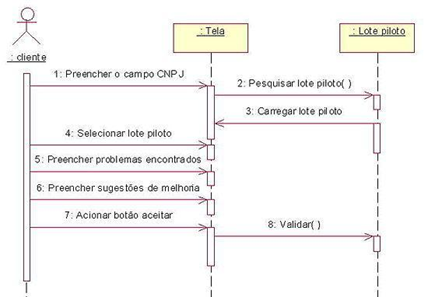
\includegraphics[scale=1.0]{imagens/DiagramadeSequencia.png}
% 	\\\textbf{Fonte:} Elaborada pelo autor
% 	\label{fig:diagramaDeSequencia}
% \end{figure}
% \FloatBarrier


% \subsection{Diagrama de Atividades}
% Havendo necessidade de detalhamento de algum procedimento, este pode ser apresentado na forma de um diagrama de atividades o qual deve ser inserido nessa seção. Podem ser elaborados quantos diagramas de atividades se fizerem necessários.


% \subsection{Diagrama de Estados}
% Sendo necessária a elaboração do diagrama de estados na fase de projeto, os novos diagramas devem ser apresentados nessa seção.


% \section{Projeto Arquitetural}
% O projeto arquitetural precede a etapa de construção da obra. O projeto arquitetural determina as partes de uma construção e como estas devem interagir. A arquitetura garante a unidade da obra, ou seja, a consistência entre as suas partes (Vergilio).

% Ver algumas definições em (Silva), sendo que um exemplo está apresentado na Figura~\ref{fig:projetoArquitetural}.


% \FloatBarrier
% \begin{figure}[!htbp]
% 	\centering
% 	\caption{Diferentes Detalhamentos dos Serviços Relacionados ao Cliente}
% 	%scale redimensiona a figura.
% 	%1.5 = 150% do tamanho original
% 	%1 = 100% do tamanho original
% 	%0.20 = 20% do tamanho original
% 	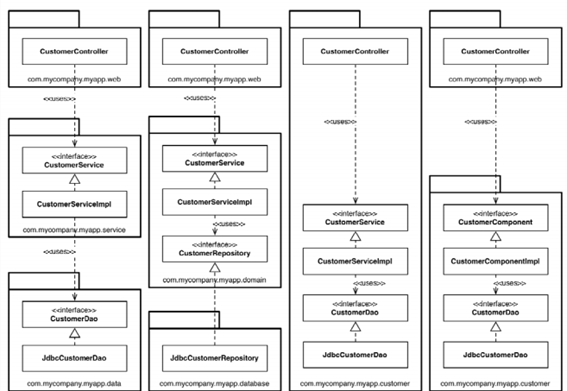
\includegraphics[scale=1.0]{imagens/ProjetoArquitetural.png}
% 	\\\textbf{Fonte:} Elaborada pelo autor
% 	\label{fig:projetoArquitetural}
% \end{figure}
% \FloatBarrier
